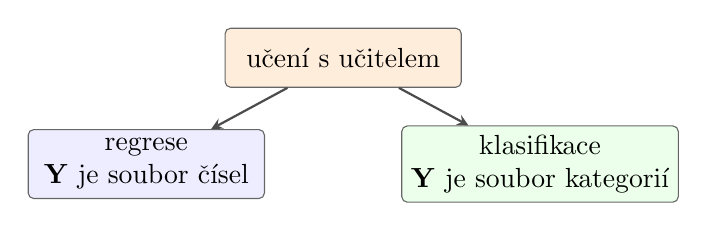
\begin{tikzpicture}[
    >=stealth,
    box/.style={
        draw=black!60,
        rounded corners=2pt,
        minimum width=3cm,
        minimum height=0.75cm,
        align=center
    },
    arr/.style={->, thick, draw=black!70}
]
    \node[box, fill=orange!14] (supervised) at (0,1.35)
        {učení s učitelem};

    \node[box, fill=blue!7] (regression) at (-2.5,0)
        {\markdarkred{regrese}\\$\mathbf{Y}$ je soubor čísel};

    \node[box, fill=green!8] (classification) at (2.5,0)
        {\markdarkred{klasifikace}\\$\mathbf{Y}$ je soubor kategorií};

    \draw[arr] (supervised) -- (regression);
    \draw[arr] (supervised) -- (classification);
\end{tikzpicture}
